\documentclass[border=5pt]{standalone}
\usepackage{pgfplots}
\pgfplotsset{compat=1.18}
\usepackage{siunitx}
\usepackage{tikz}
\usetikzlibrary{calc}

\definecolor{trainColor}{RGB}{31,119,180}
\definecolor{valColor}{RGB}{255,127,14}

\begin{document}
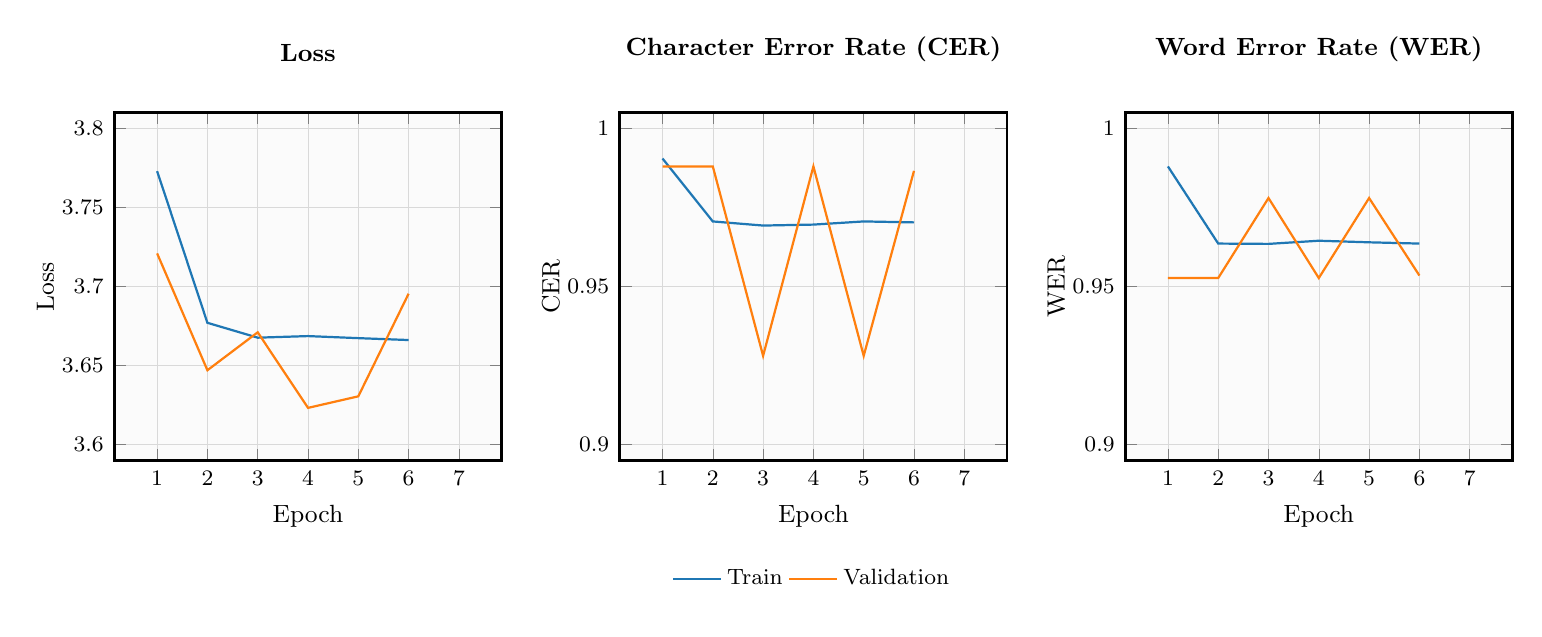
\begin{tikzpicture}[remember picture]

    % Graph 1: Loss
    \begin{axis}[
        name=plot1,
        width=6.5cm,
        height=6cm,
        xlabel={Epoch},
        ylabel={Loss},
        ylabel style={yshift=-0.15cm},
        xmin=0.5, xmax=7.5,
        ymin=3.6, ymax=3.8,
        xtick={1,2,3,4,5,6,7},
        grid=both,
        grid style={line width=.1pt, draw=gray!10},
        major grid style={line width=.2pt,draw=gray!30},
        title={Loss},
        axis background/.style={fill=gray!3},
        title style={yshift=3mm, font=\small\bfseries},
        label style={font=\small},
        tick label style={font=\footnotesize},
        line width=1pt,
        enlarge x limits=0.05,
        enlarge y limits=0.05,
        every axis plot/.append style={no markers},
        legend to name=commonlegend,
        legend columns=2,
        legend style={draw=none, fill=none, font=\footnotesize}
    ]
        % Train
        \addplot[color=trainColor, thick] coordinates {
            (1, 3.7730) (2, 3.6771) (3, 3.6677) (4, 3.6687) (5, 3.6674)
            (6, 3.6662)
        };
        
        % Validation
        \addplot[color=valColor, thick] coordinates {
            (1, 3.7210) (2, 3.6471) (3, 3.6711) (4, 3.6233) (5, 3.6306)
            (6, 3.6955)
        };
        
        \legend{Train, Validation}
    \end{axis}
    
    % Graph 2: CER, positioned to the right of plot1
    \begin{axis}[
        name=plot2,
        at={($(plot1.east)+(1.5cm,0)$)},
        anchor=west,
        width=6.5cm,
        height=6cm,
        xlabel={Epoch},
        ylabel={CER},
        ylabel style={yshift=-0.15cm},
        xmin=0.5, xmax=7.5,
        ymin=0.9, ymax=1.0,
        xtick={1,2,3,4,5,6,7},
        grid=both,
        grid style={line width=.1pt, draw=gray!10},
        major grid style={line width=.2pt,draw=gray!30},
        title={Character Error Rate (CER)},
        axis background/.style={fill=gray!3},
        title style={yshift=3mm, font=\small\bfseries},
        label style={font=\small},
        tick label style={font=\footnotesize},
        line width=1pt,
        enlarge x limits=0.05,
        enlarge y limits=0.05,
        every axis plot/.append style={no markers}
    ]
        % Train
        \addplot[color=trainColor, thick] coordinates {
            (1, 0.9905) (2, 0.9706) (3, 0.9693) (4, 0.9696) (5, 0.9706)
            (6, 0.9703)
        };
        
        % Validation
        \addplot[color=valColor, thick] coordinates {
            (1, 0.9880) (2, 0.9880) (3, 0.9281) (4, 0.9880) (5, 0.9281)
            (6, 0.9866)
        };
    \end{axis}
    
    % Graph 3: WER, positioned to the right of plot2
    \begin{axis}[
        name=plot3,
        at={($(plot2.east)+(1.5cm,0)$)},
        anchor=west,
        width=6.5cm,
        height=6cm,
        xlabel={Epoch},
        ylabel={WER},
        ylabel style={yshift=-0.15cm},
        xmin=0.5, xmax=7.5,
        ymin=0.9, ymax=1.0,
        xtick={1,2,3,4,5,6,7},
        grid=both,
        grid style={line width=.1pt, draw=gray!10},
        major grid style={line width=.2pt,draw=gray!30},
        title={Word Error Rate (WER)},
        axis background/.style={fill=gray!3},
        title style={yshift=3mm, font=\small\bfseries},
        label style={font=\small},
        tick label style={font=\footnotesize},
        line width=1pt,
        enlarge x limits=0.05,
        enlarge y limits=0.05,
        every axis plot/.append style={no markers}
    ]
        % Train
        \addplot[color=trainColor, thick] coordinates {
            (1, 0.9880) (2, 0.9636) (3, 0.9635) (4, 0.9645) (5, 0.9640)
            (6, 0.9636)
        };
        
        % Validation
        \addplot[color=valColor, thick] coordinates {
            (1, 0.9527) (2, 0.9527) (3, 0.9780) (4, 0.9527) (5, 0.9780)
            (6, 0.9535)
        };
    \end{axis}

    % Positioning the common legend below all graphs
    \node at ($(plot1.south)!0.5!(plot3.south)+(0,-1.5cm)$) {\pgfplotslegendfromname{commonlegend}};
    
\end{tikzpicture}
\end{document}